% !TeX program = lualatex
% Using VimTeX, you need to reload the plugin (\lx) after having saved the document in order to use LuaLaTeX (thanks to the line above)

\documentclass[a4paper]{article}

% Expanded on !p snip.rv = get_formatted_date() at !p snip.rv = get_formatted_time().

\usepackage{style}

\title{SHS Innovation et energie}
\author{Arthur Herbette}
\date{Mardi 16 septembre 2025}

\begin{document}
\maketitle

\section{Sources fossiles}

\lecture{2}{2025-09-16}{Energie fossile}{}


\begin{parag}{La géologie des sources fossiles}
	L'extraction du pétrole/gaz peut se faire de plusieurs façons, on peut aller de EROI $\approx 7 \to 35$
    \begin{subparag}{EROI}
        Imaginons que nous prenons 100MJ de pétrole, l'extraction nous coûte 10Mj, raffiner 27MJ, le transport nous coûte 5MJ, le dernier coût qui est le coût energetique des infrastructure nous revient à 37.5MJ On fini donc
	\begin{align*} 100 \to 90 \to 63 \to 58 \to 20.5 \end{align*}
	\begin{align*} \text{Pétrole restant à la consomation} = 20.5MJ \text{ oil} \end{align*}
	\begin{framedremark}
	Même dans ce calcul il manque encore pas mal de donnée, notamment l'installation etc...
	\end{framedremark}
	\begin{framedremark}
	Comme par exemple vouloir mettre des panneauc solaires dans l'espace,cela paraît être une bonne idée au vu de l'ensoleillement mais l'installation...
	\end{framedremark}
    \end{subparag}
\end{parag}


\begin{parag}{Courbe de Hubbert}
    Avec la technique d'exploitation qui s'améliore, la recherche augmente, néanmoins la ressource n'est pas infini fait baisser la production.
\end{parag}

\begin{parag}{Effet sur le climat et l'environnment}
    Reaction de combustion d'un hydrocarbure générique a l'air libre en présence d'azote $N_2$
    \begin{align*} C_xH_y + z(O_2) + 3.77N_2 \to x(CO_2) + (y\2)(H_2O) \end{align*}
    \begin{subparag}{Exemple}
        Combien de $CO_2$ est relaché par la combustion du ccharbon?
	\begin{align*} C + O_2 \to CO_2 \\
	[12] +  [2 x 16] \to [44]\end{align*}
	chaque kilo de charbon libère 44/12~3.67 kg de $CO_2$
	\begin{itemize}
		\item Si l'on considère du charbon bitumineux avec une teneure de 10 en volatile (eau), il reste 900kg de combustible par tonne de charbon
		\item Si 88\% du combustible sec est centres, soit du charbon pur, il reste 900 x 0.88 = 792 kg de charbon, ce qui nous donne 3.67 x 792 ~2910kh = 2.81 tonne de $CO_2$ par tonne de charbon
		\item valeur energetique ~35Gj/tonne + un rendement ~30 \%, on produit environ 35 * 0.3 ~ 10.5Gj électrique ~2.92 MWh par tonne de charbon.
	\end{itemize}
	
    \end{subparag}
\end{parag}
\begin{parag}{est ce qu'il y aurait un lien directe entre les grand pétroliers et les grandes canicules (heatwaves)}
	Ce qu'on voit après une analyde des graphes (raccourcis btw) Oui par exemple Saudi Aramco est reponsable à 19\% de l'augmentation de 0.05-0.10 degrés.  
    \begin{subparag}{Est ce que les petrolier savaient pour le changement climatique}
        Oui, des chercheurs directement travaillant sur les petroliers savait que l'utilisation des energie fossile augmente la température globale.
    \end{subparag}
\end{parag}

\begin{parag}{Compensation des émissions}
    Une entreprise venant de pays industrialisé (imaginons l'italie) peut acheter des "droite de pollutions" à la place du pays peu développer. On a donc un commerce des émissions de carbone.
\end{parag}

\begin{parag}{Chauffage par mazout}
Solution pour aider la transition:
\begin{itemize}
    \item Commencer par les \textbf{grand bâtiments} publique car l'investissment est plus rentable (volume >>> pour s >)
    \item Comment faire opur inciter: mettre des taxes carbonnes
    \item Faciliter les emprunts
\end{itemize}
Economies de $CO_2$: le polyuréthane est un matériel isolant produit par la pétrochimie - pas de pétrole $\to$ pas de polyuréthane!!\\
Quel est le cout $CO_2$ de la production du polzuréthane?\\Cela dépends de la source qu'on considère.\\
Peut être une solution serait d'utiliser un materiel isolant plus vert du genre: Liège, paille, laine? Ils sont aussi beaucoup plus couteux, mais leur impact $CO_2$ de production est beaucoup plus petit...\\
\begin{framedremark}
Par exemple le projet REBUILT project ENAC/EPFL fait à l'epfl
\end{framedremark}
Maintenant est ce que la production des ces matériaux est suffistant et faisable?
\begin{subparag}{et si on ajoutait une pompe à chaleur}
    Si on reprendre une pièce que l'on veut maintenant à 20C, alors l'amortissement du prix d'installation ce fait en environ 830 jours.\\
    \begin{itemize}
	    \item Installation 10'000CHF
	    \item Radiateur electrique 15.5
	    \item Pompe à chaleur 4
    \end{itemize}
    
\end{subparag}
\end{parag}
\begin{parag}{Economies d'énérgie: transport}
    La question maintenant est, est ce qu'on peut faire des économies d'énérgie sur le transport. 
    \begin{itemize}
	    \item Projet de remiédation SwissLoop de EPFZ/EPFL
    \end{itemize}
    On a que la voiture est à environ 580 Wh/passager * km, tandis que le tgv et autre train se trouve vers les 200
    
\end{parag}






\begin{parag}{Transport routier sans $CO_2$: bioéthanol}
	Quelle surfacec dois-je couvrir en champs de mais pour la production de bioéthanol pour alimenter tous le transport routier en Suisse pendant 1 an?\\
	Il faudrait environ 0.6\% de la surface totale de la Suisse.
	\begin{itemize}
		\item L'intégralité du reseau autoroutier Suisse a une longueur L1 ~1'700km
		\item L2 = $S_{mais}$/ L1~150m
	\end{itemize}
\end{parag}
\begin{parag}{Voiture électrique/hybride}
	Faisons un cas d'étude entre deux VWs:
    \begin{itemize}
	    \item Cout énergetique de la voiture
		    \begin{itemize}
			    \item Extraction et preparation de la matière première, similaire pour les 2x VWs
			    \item Manufacture, similaire pours les 2x
			    \item Porduction de la batterie
			    \item Utilisation , consommation
			    \item Recyclage
		    \end{itemize}
		    
		    \item Calcul du $CO_2$ total en fonction du mix énergétique
		    \item Dscussion des hypothèses 'techniques' (énergie et $CO_2$)
		    \item Resultats: extra slides et fichier Excel éditable sur Moodle
    \end{itemize}
    
\end{parag}

	
\begin{parag}{Résumé - les sources fossiles}
Le seul scénario qui permet la baisse de l'energie fossile est de ne \textbf{PLUS} ouvrir aucun gisement. Ce derniers scénarion n'est pas vraimment acceptable par l'économie actuelle, la baisse de production de ses sources fossiles rendrait la population la première victime de cet arrêt de production.
\end{parag}
\subsection{Conclusion}
    La transition énergétique/écologique est essentielle, dans un format scientifiquemenet et techniquement réaliste et réalisable dans les prochaines trentes années.\\
    Le problème principale à résoudre et remplacerenviron 80\% de l'énergie fossile actuellement utiliser


\section{Transition énergétique}
    
\begin{parag}{Vision d'ensemble des flux d'énergie}
	\begin{subparag}{Potentiel}
	    On voit bien que l'énergie potentiel du solaire arrive à 4 ordre de grandeur de différence avec les autres énérgie renouvable, le nucléaire arrive lui à 2/3 ordre de grandeurs ce qui est largement suffisant pour l'humanité acutelle.
	\end{subparag}
    
\end{parag}

\begin{parag}{Conecept de densité de puissance}
    Cherchons par exemple combien de w par $m^2$  à t'on besoin pour produire du bioéthanol, On obtient donc:\\
    Soyons optimiste: aucune perte d'efficacitl + tout le mais produit en CH est utilisé
    \begin{align*} 35 \cdot 1'200 \cdot 31'536 \cdot  10'000 = 0.13 \mathspace \left[\frac{W}{m^2}\right] \end{align*}
\begin{itemize}
	\item vent ~ 10/100 w/$m^2$
		\item hydro ~ rip
\end{itemize}

\end{parag}

\begin{parag}{Estimer la densité de puissnace produite par des éoliennes}
	On a que l'énergie est donnée environ par:
	\begin{align*} E = f \cdot  \frac{1}{2}\rho Sv^2L \end{align*}
	Ou alors, la puissance est donnée par:
	\begin{align*} P = \frac{E}{t} = f \cdot  \frac{1}{2}\rho Sv^3 \end{align*}
	Néanmoins ici on en prends pas en compte le mecanical load qui nous fait perdre encore de l'énergie\\
   \begin{subparag}{Roles de la turbulence}
       Un effet très important de la turbulence qui affect le régime en flux laminaire de l'air\\
       Une conséquence principale de tourbillons produits par les pales de l'éolienne: il faut séparer les éoliennes de $5d$ où d est la longueur d'une pale
   \end{subparag} 
\end{parag}
\begin{parag}{Energie solaire}
    Sur un an le rayonnement solaire sur la Suisse est 220 fois plus élevé que la consommation d'énergie
    \begin{subparag}{énergie quntique- photovoltaique}
        \begin{itemize}
		\item effet photo-électrique: un photon tape sur la matière et produit un électron libre, capable de migrer
		\item effet photo-voltaique: un photon qui tape dans un semi conducteur (sillicium) produit une paire electron-trou, qui dans un potentiel électrique génère un courent $\to$ énergie
		\item Rendement total de ce cycle: $\frac{\text{énergie électrique}}{\text{énergie lumineuse}} = 10\%$
        \end{itemize}
        
    \end{subparag}
\end{parag}
\begin{parag}{Densité de puissance solaire: l'ensoleillement moyen sur l'année}
    \begin{align*} P_{grid} = P_{earth} \cdot  \nu_{PV} \cdot  FR \end{align*}
    le $FR$ est le facteur de recouvrement améliiorable avec miroirs - solaire à concentration
\end{parag}
\begin{parag}{Intégration technologique: panneaux solaires flottants sur barrage hydro.électrique}
	\begin{itemize}
		\item ~400W / $m^2$  en Suisse ~220 fois plus que la consommation annuelle totale d'énergie\Rendement d'un panneaux solaire thermique
			\begin{align*} \nu_{PV} =  \nu_0 - \alpha \Delta T_{ext} \frac{T_{EXT}^2}{G} \end{align*}
	\end{itemize}
	
    
\end{parag}
\begin{parag}{Problème}
    Par rapport au celluls PV standard en silicium les celluls en pérovskite souffrent de problmes de vieillissement et de stabilité structurale (résistance à l'humidité, par exemple) à l'echelle industrielle du module\\
    Etude de l'EPFL à 2017: durée  de vie 12'000 heure.
\end{parag}







\lecture{3}{2025-09-23}{oui}{}
\subsection{Fin de l'impact de l'énergie sur la société}

\begin{parag}{Effet Rebond}
    \begin{definition}
        En trouvant une solution au problème la solution finalement empire ce problème
    \end{definition}
    \begin{subparag}{Exemple}
        Par exemple, vouloir manger moins de calorie en mangant de la glace basse en calorie mais ducoup en manger plus car moins calorique $\to$ plus de calorie au final.
    \end{subparag}
\end{parag}
\begin{parag}{Evolution de la consommation finale d'energie}
	\begin{center}
    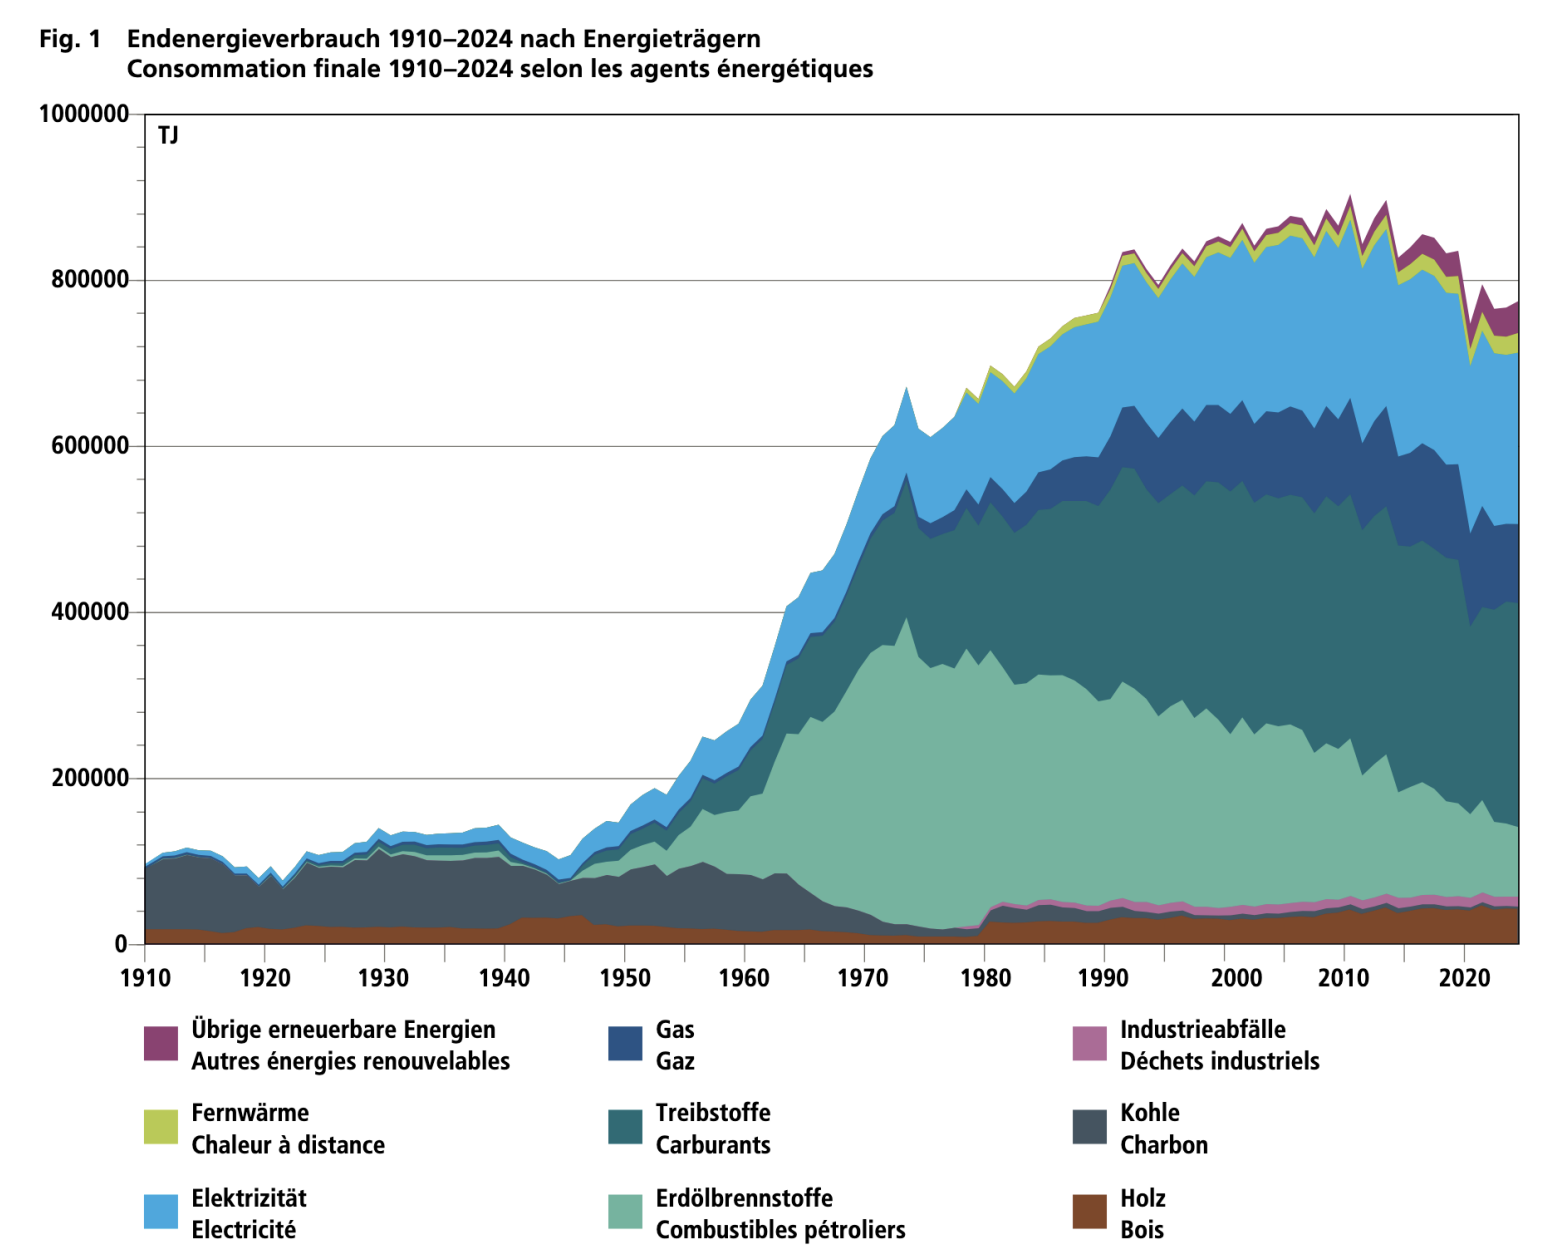
\includegraphics[scale=0.2]{12025-09-23.png}
	\end{center}
	
    On voit ici que cet emmissions est seulement au niveau locale (production sur le terrain Suisse) néanmoins beaucoup de la production est délocalisé de nos jours ce qui expliquer pourquoi la production peut baisser.
\end{parag}
\begin{parag}{Energie primaire, secondaire, finale, utile}

	\begin{center}
   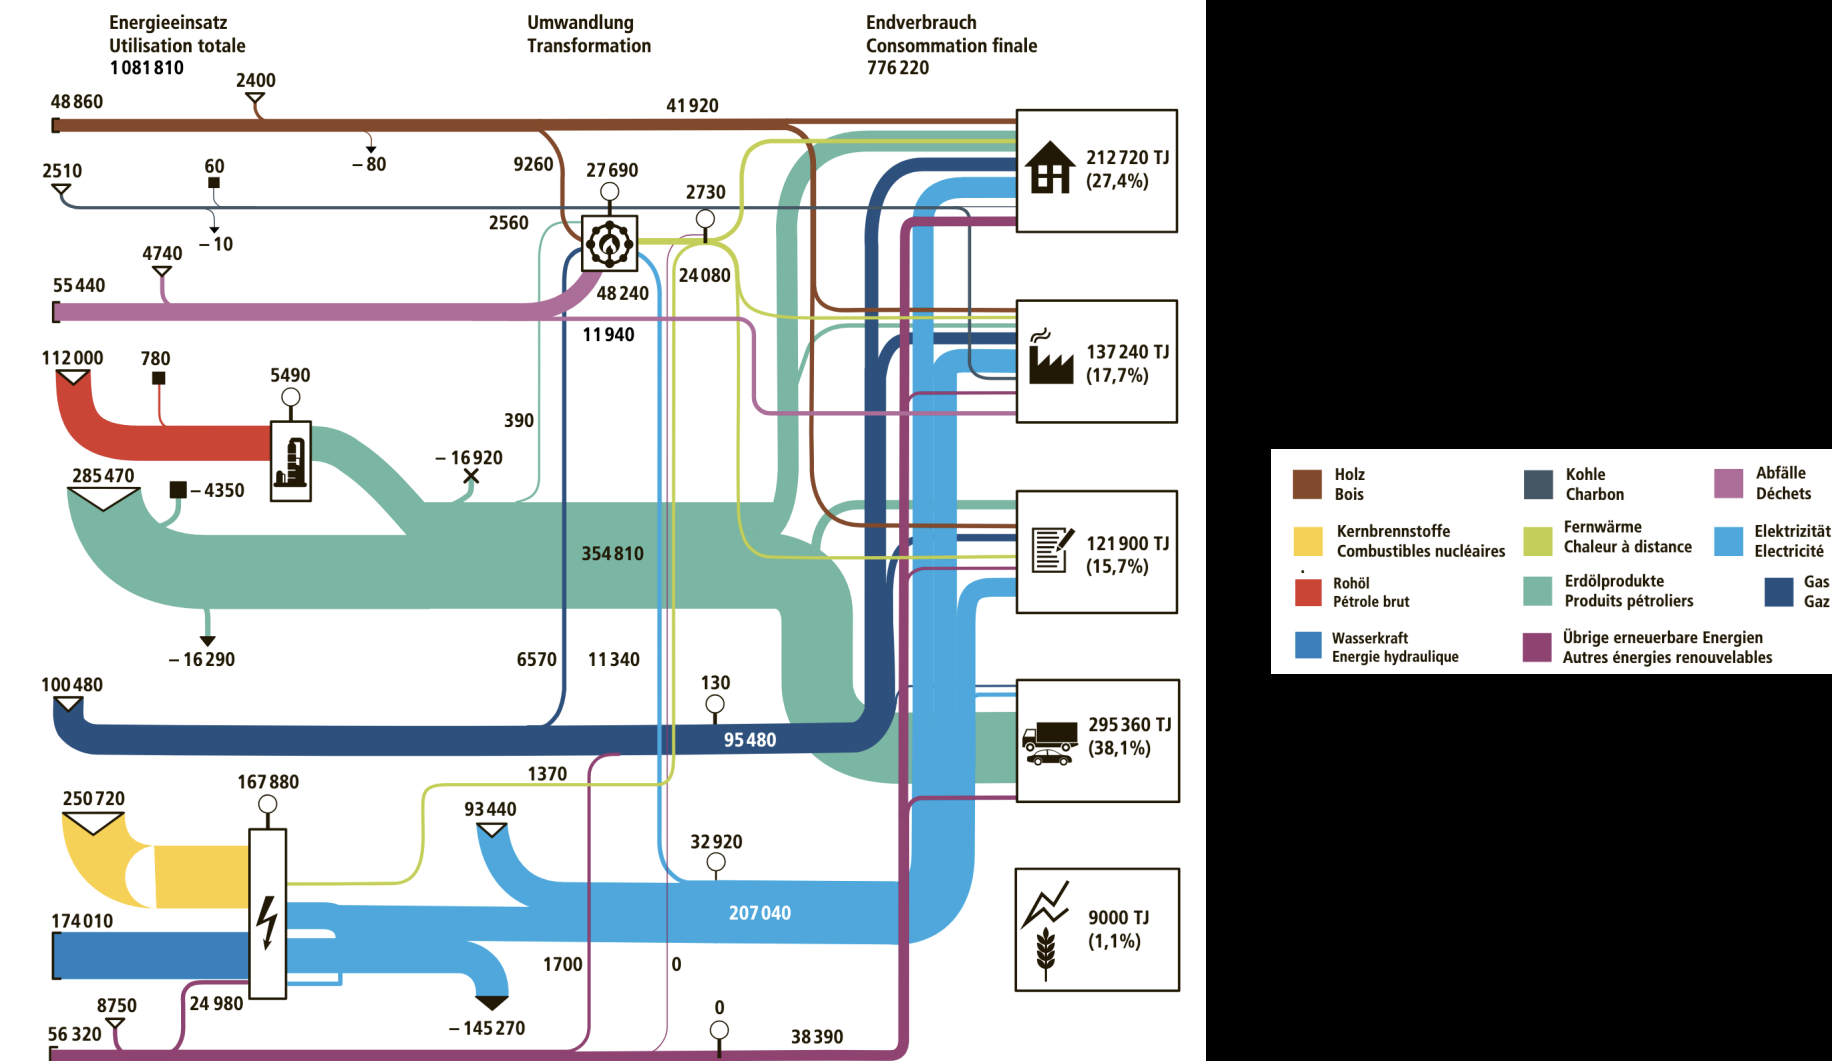
\includegraphics[scale=0.2]{22025-09-23.png} 
	\end{center}
	
\end{parag}



\begin{parag}{Pourquoi continue t-on à chercher?}
	\begin{center}
	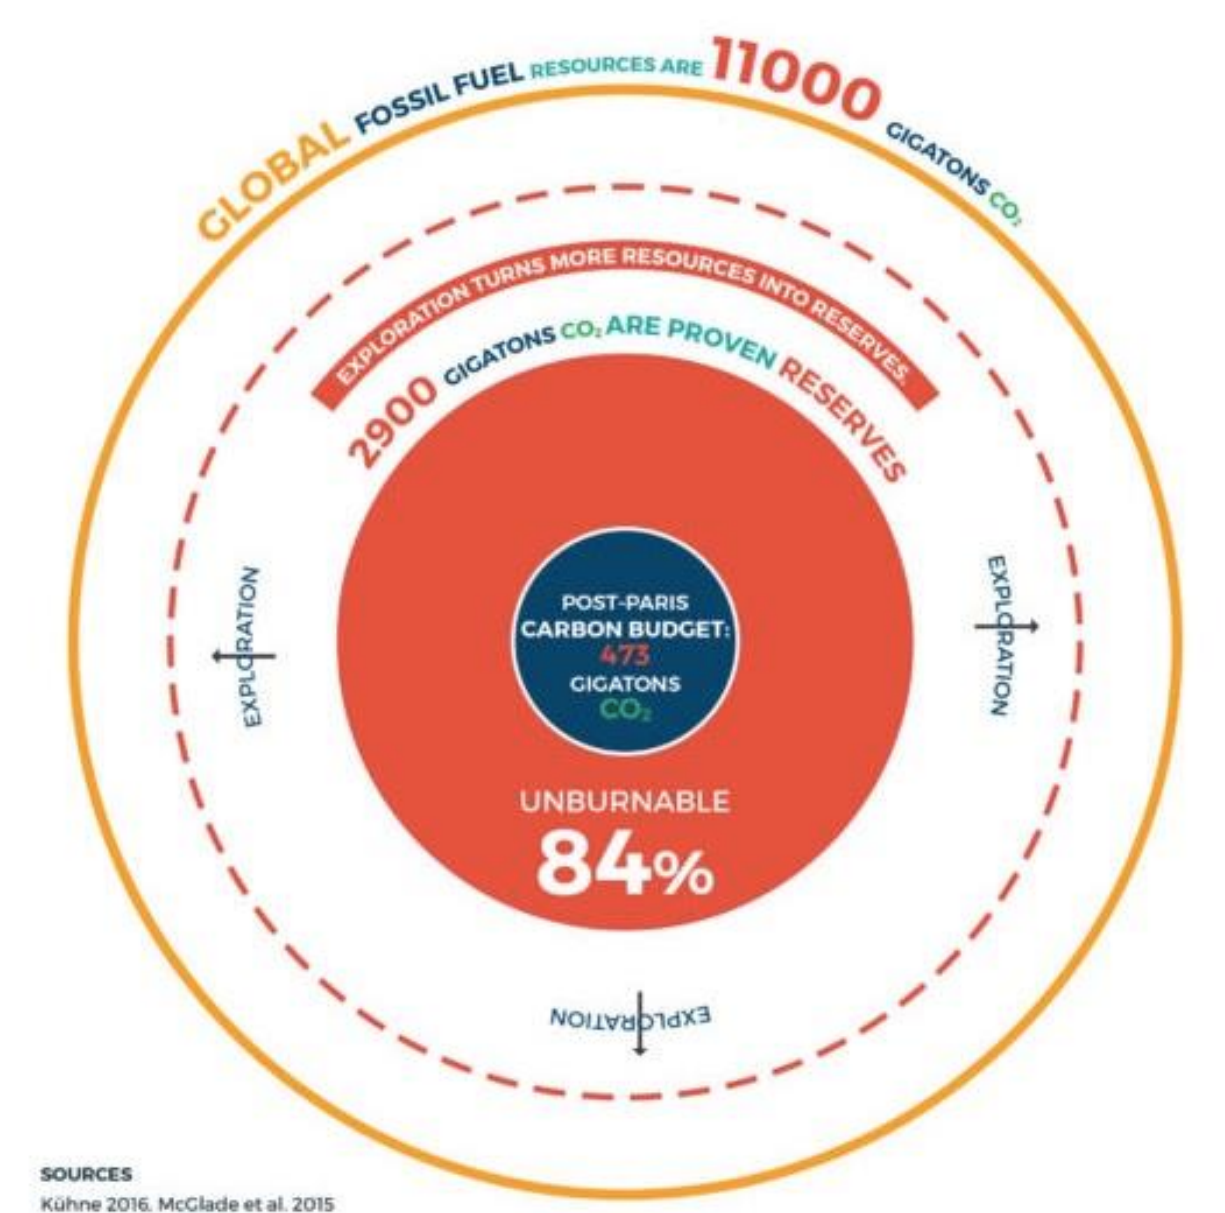
\includegraphics[scale=0.2]{42025-09-23.png}
	\end{center}
	
    Donc ici par rapport aux accord de paris (au maximum 2 degrés de réchauffement). Si on brûle toute la reserve de pétrole qu'on a, il y en a 84\% qui sont en surplus\\
    Ici ce qui est important c'est pas vraimment le stock mais plus le \important{flux}

\end{parag}
\begin{parag}{EROI des dlcouvertes (aux USA)}
	\begin{center}
	    
	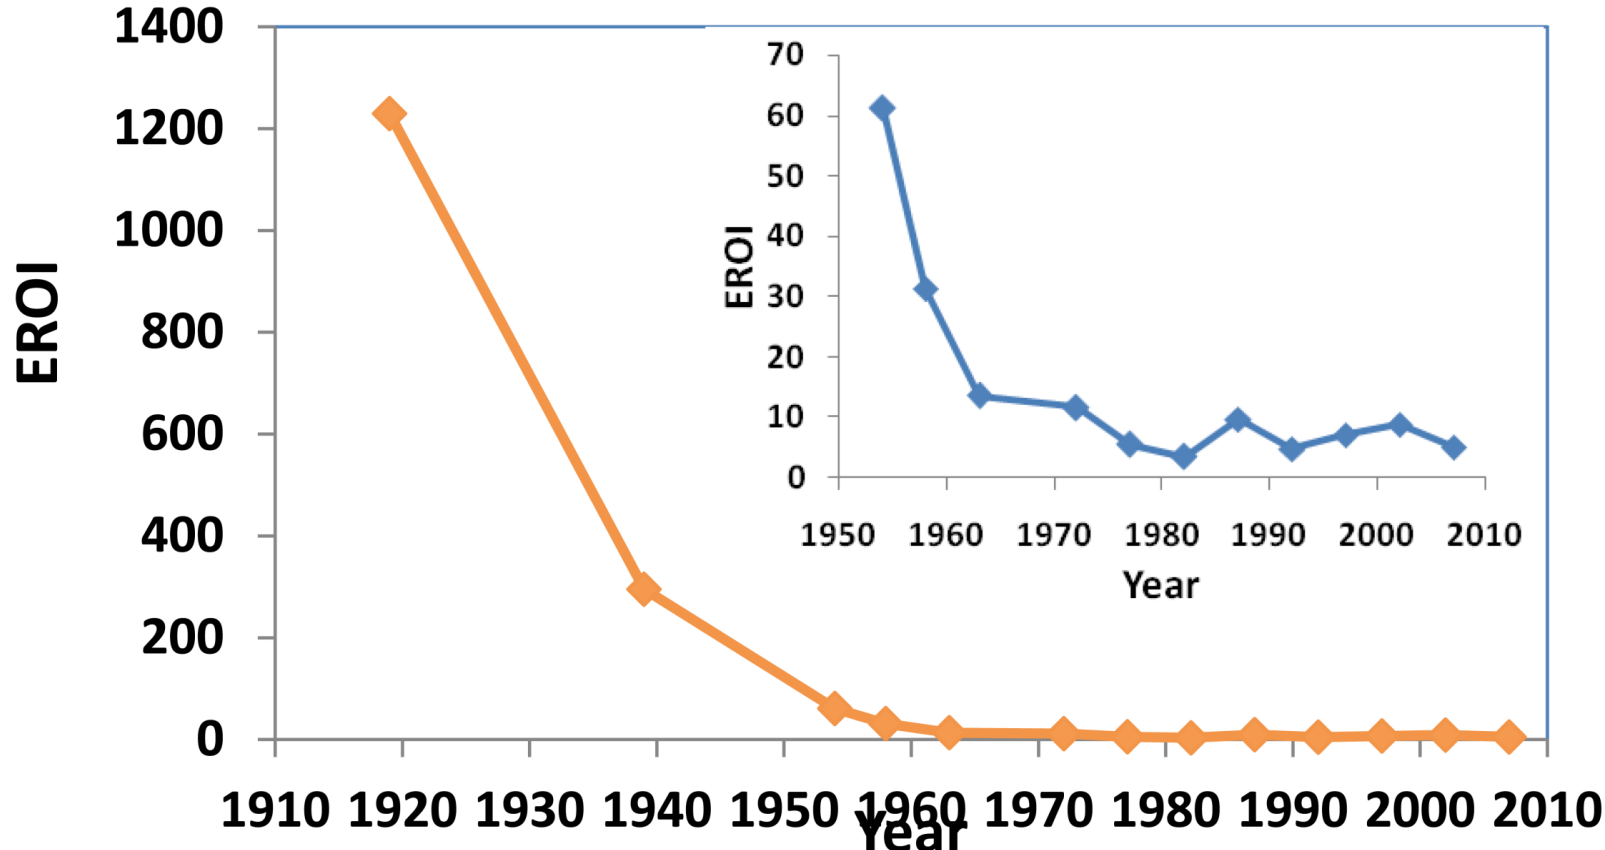
\includegraphics[scale=0.2]{62025-09-23.png}
	\end{center}
	
	On voit ici, lors de la découverte d'un champs c'est souvent les endroits les plus intérressant et les plus facile pour extraire, dès lors on voit que le ROI descend car la facilité d'extraction diminue
    
\end{parag}
\begin{parag}{EROI de la production}
	\begin{center}
	    
	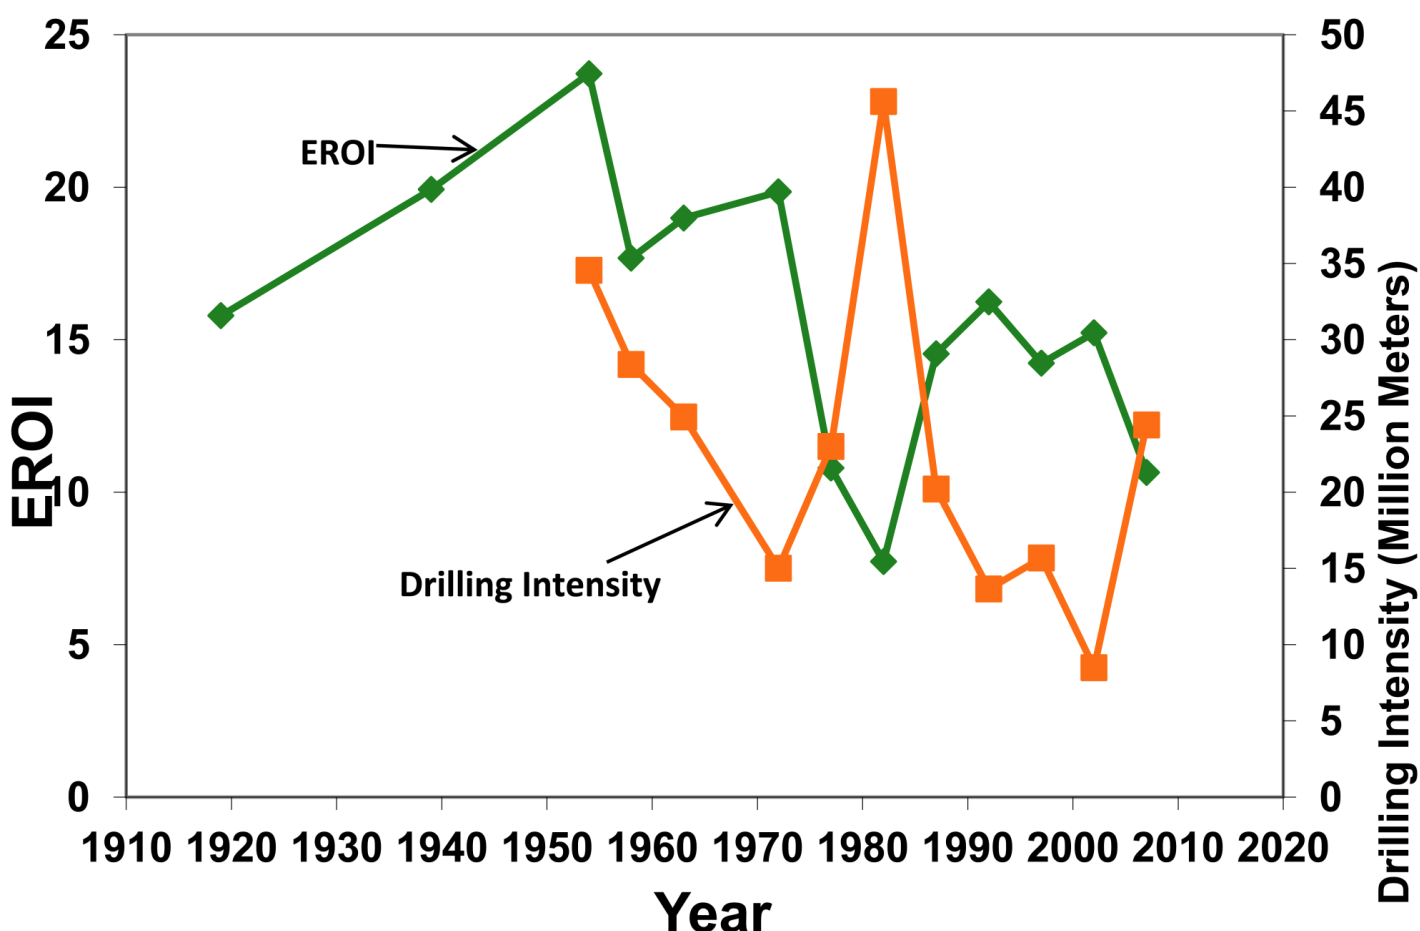
\includegraphics[scale=0.2]{72025-09-23.png}
	\end{center}
	
	Lorsqu'on pompe beaucoup, on va dans des champs qui sont moins bons ce qui donc fait descendre le flux
    
\end{parag}


\subsection{Innovation durable}

\begin{parag}{Différence entre Créativité Innovation Progrès}
	\begin{subparag}{Créativité}
	    Jouer avec ses idées
	\end{subparag}
	\begin{subparag}{Innovation}
	    Generer du profit grâce à sa  créativité $\to$ impact économique
	\end{subparag}
	\begin{subparag}{Progrès}
	    Avoir un impact positif sur la société $\to$ impact sociétal
	\end{subparag}
	\begin{subparag}{Aparté sur l'innovation}
	    Opower (jsp c'est quoi) on voulu faire baisser la consommation d'un habitat. Il voulait le faire en changeant la \important{mentalité des gens} et non la technologie. Par exemple un dashboard de l'argent économisé, ou alors nous faire être sauveur de la planête.\\
	    Le \important{plus rentable}: avoir une compétition entre les voisins, avoir un classement entre les voisins
	\end{subparag}
	\begin{framedremark}
	Par exemple avoir un quartier sans panneau photovoltaique, dès qu'une personne en mets $\to $ effet boule de neige vers le quartier.
	\end{framedremark}
\end{parag}


\begin{parag}{Buisness model canva}
	\begin{center}
    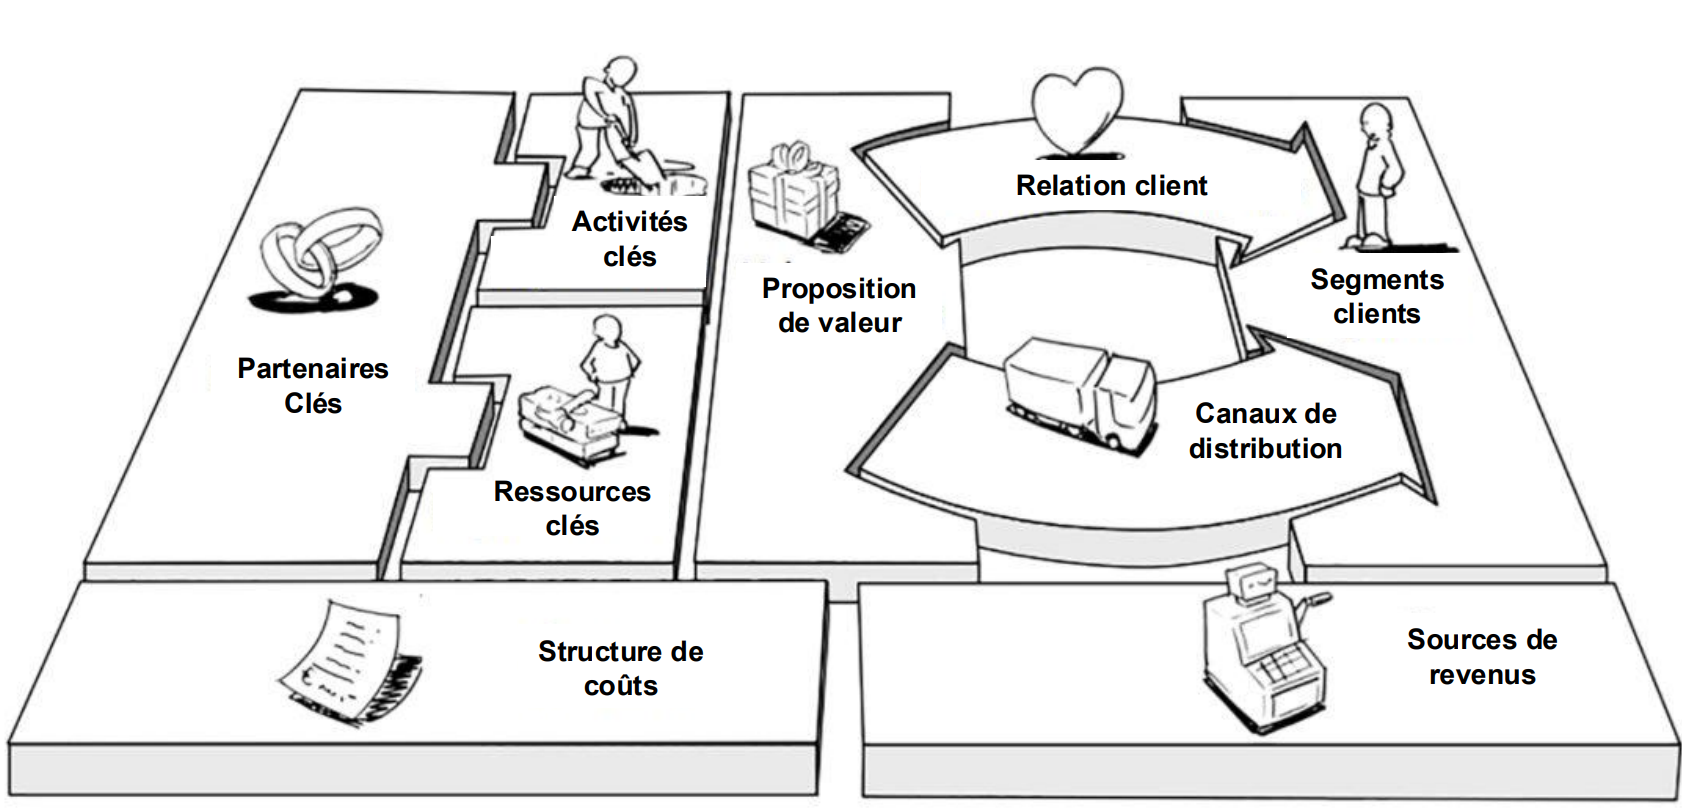
\includegraphics[scale=0.2]{82025-09-23.png}
	\end{center}
	
    \begin{itemize}
	    \item Est ce que c'est faisable?
	    \item Est ce qu'il est viable, revenu $>$ coût?
	    \item Est ce qu'il est désirable? Est ce que des gens veulent acheter votre produit
    \end{itemize}
    
\end{parag}


\begin{parag}{Maslow}
	\begin{center}
    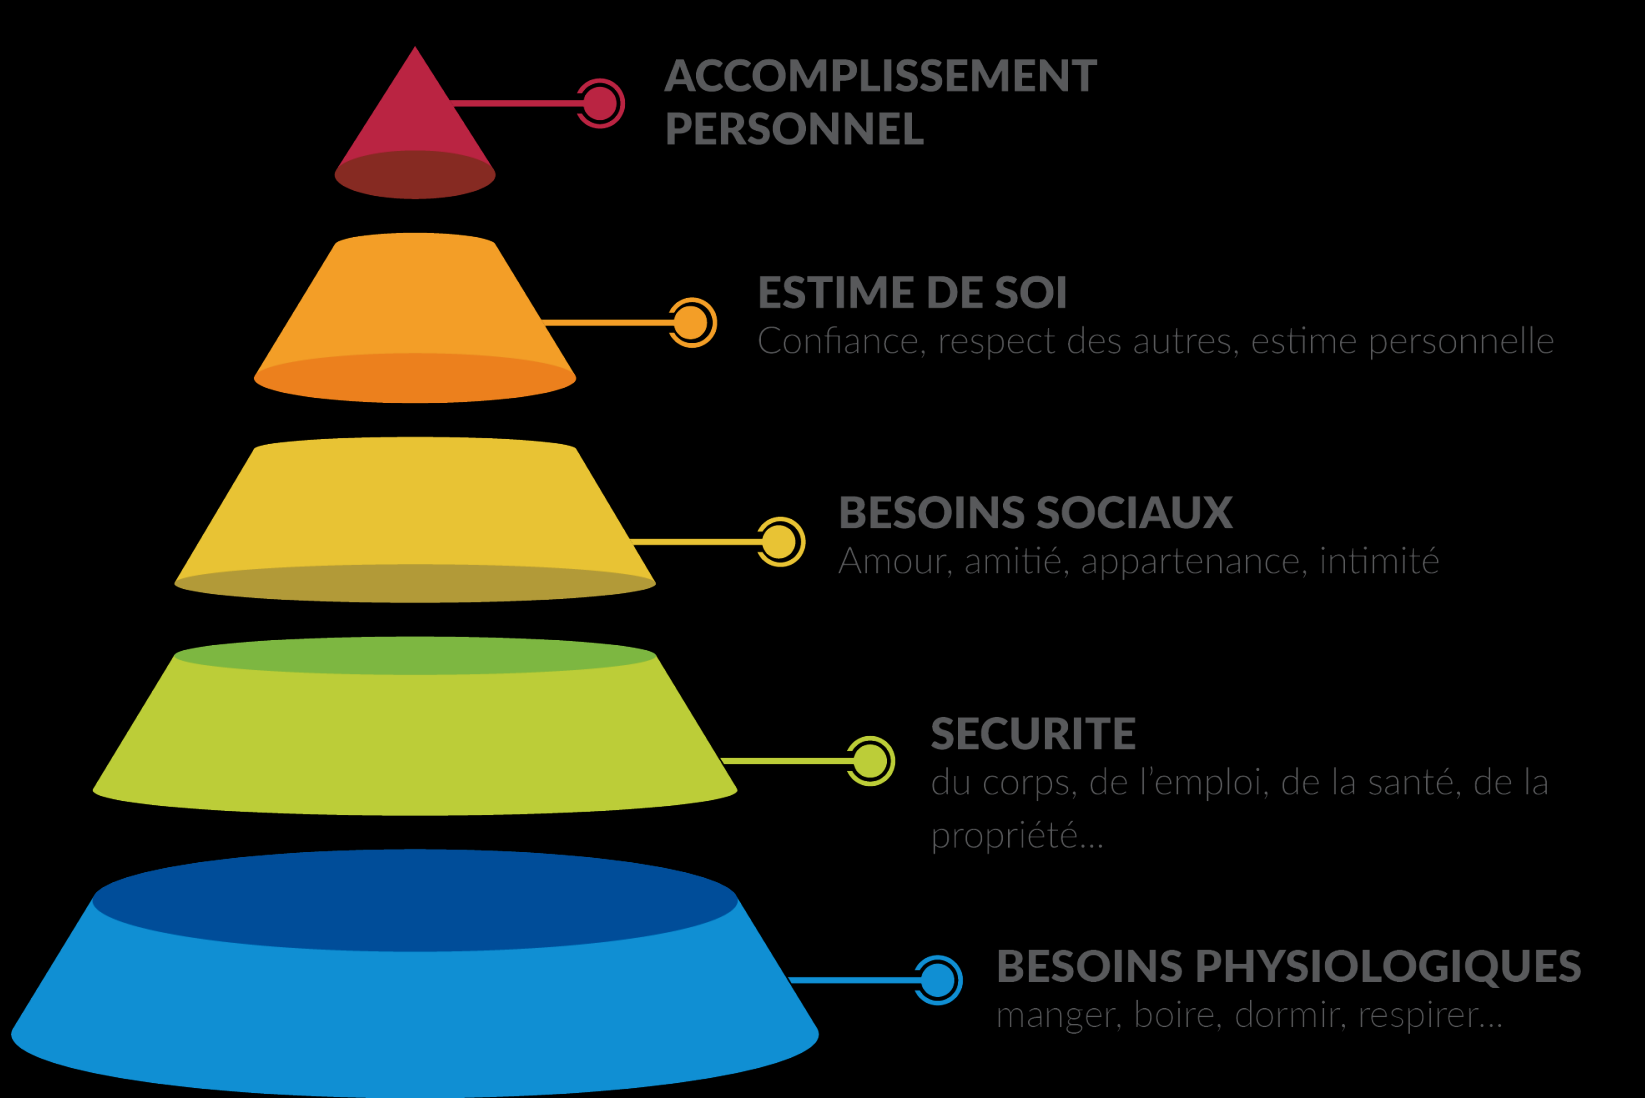
\includegraphics[scale=0.15]{92025-09-23.png}
	\end{center}
	
    Ici on parle des besoins les plus primitifs dans une société jusqu'à ce qui est le moins "nécessaire"\\
    On a plus vraimment de besoin mais plus de désir.\\
    \begin{center}
    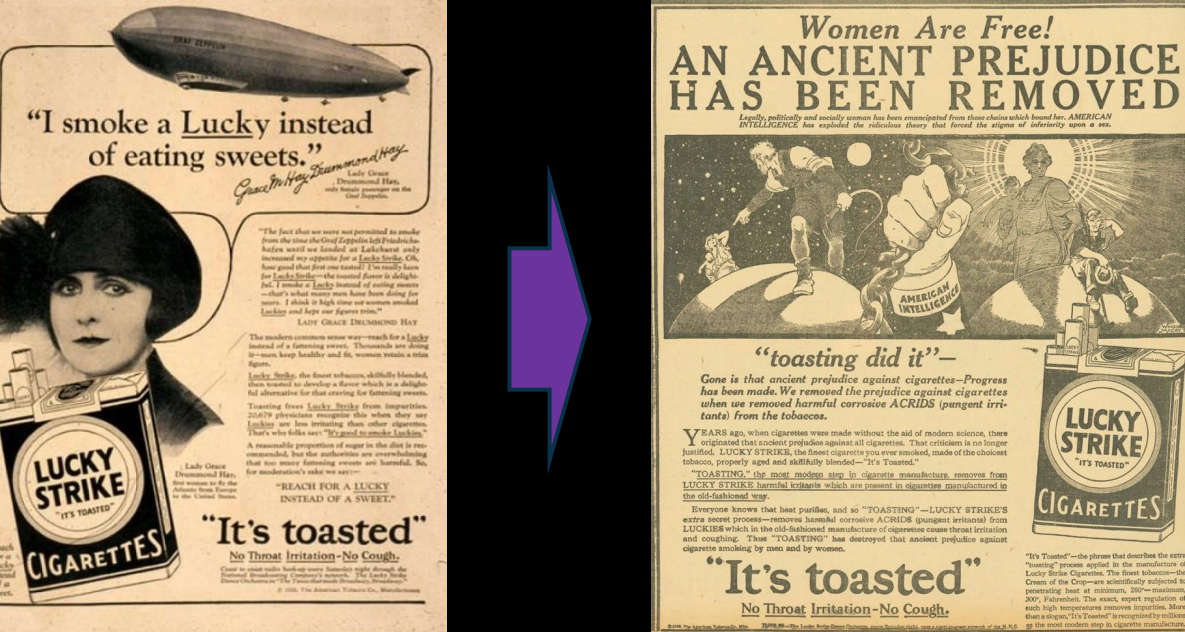
\includegraphics[scale=0.2]{102025-09-23.png}
    \end{center}
    
    Par exemple la cigarette chez les femmes au états unis. Les femmes de l'époques de fumait pas, c'était mal vu. Edward Bernays a alors amené la cigarette comme un produit faisant. La cigarette est aussi devenu un signe de feminisme chez les femmes américaines de l'époque. Grâce à ces deux images la cigarette est devenue populaire aussi chez les femmes.\\
    On voit encore une fois qu'on est passé d'une économie de besoin à une économie de désir.
\end{parag}


\subsection{Robustesse et flexibilité}
\begin{parag}{Prix des technologies}
    Imaginons que nous ayons les quatre intallations éolienne, gaz, nucléaire, hydraulique, quelles sont les problèmes respectifs de chacunes des installations:
    \begin{itemize}
	    \item Eolienne: pas flexible (depend du temps)
	    \item Gaz: flexible
	    \item Nucléaire: flexible, coût si l'on doit arreter
	    \item Hydraulique: très flexible
    \end{itemize}
    Maintenant quelle est le coût:
    \begin{align*} \text{Coût investissement} \approx \frac{\text{investissement initial}}{\text{Energie théorique sur l'ensemble du cycle de vie}} \end{align*}
    
    \begin{align*} \text{Coût carburant ou carbonne} \approx \frac{\text{cout carburant ou carbonne}}{\text{energe generé}} \end{align*}
    \begin{align*} \text{Cout o M}\approx \frac{\text{count annuel des salaires}}{\text{Energie théorique générée durant l'année}} \end{align*}
\end{parag}
\begin{parag}{installations}
	\begin{subparag}{Gaz}
	    Max $1MWh$ chaque période
	\end{subparag}
	\begin{subparag}{Nucléaire}
	    Coût d'arrêt de la centrale
	    \begin{itemize}
		    \item 100CHF
		    \item Max $1MWh$ chaque période
	    \end{itemize}
	    
	\end{subparag}
   \begin{subparag}{Hydro: Accumulation}
	   La production est flexible $1MWh$ stocké (peut produire sur une période seul)
   \end{subparag} 
   \begin{subparag}{Eolien}
       Production intermittente:
       \begin{align*} 17-18MWh \mathspace \mathspace 18-19:0MWh \mathspace \mathspace 19-20:MWh \end{align*}
   \end{subparag}
\end{parag}

\begin{parag}{Coût par installation}
    \begin{center}
    \begin{tabular}{|c|c|c|c|c|}
	    \hline
	    & Eolien & Nucléaire & hydraulique & Gaz \\
	    \hline
	    \hline
	    Investissement  & 38 & 11 & 35 & 9 \\
	    \hline 
	     Démantèlement& 0 & 0 & 0 & 0 \\
	    \hline 
	     Carburant& 0 & 9 & 0 & 46 \\
	    \hline 
	     Carbon& 0 & 0 & 0 & 10 \\
	    \hline 
	     O \& M & 18 & 13 & 5 & 6 \\
	    \hline 
    \end{tabular}
    \end{center}
    
\end{parag}







\end{document}
